\documentclass{article}
\usepackage{tikz}
\usetikzlibrary{positioning}

\begin{document}

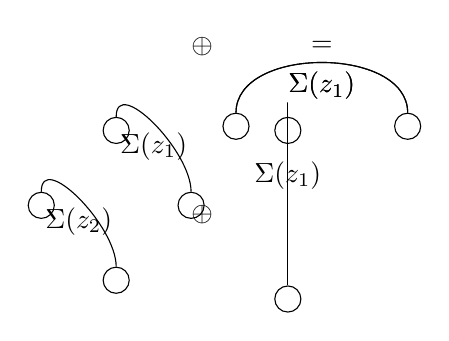
\begin{tikzpicture}[node distance=1cm]
    \node (n1) [circle,draw] {};
    \node (n2) [circle,draw,below right=of n1] {};
    \node (n3) [circle,draw,below left=of n2] {};
    \node (n4) [circle,draw,below left=of n1] {};
    
    \draw (n1) to[out=90,in=90] node[below] {$\Sigma(z_1)$} (n2);
    \draw (n3) to[out=90,in=90] node[below] {$\Sigma(z_2)$} (n4);
    
    \node (oplus1) [above right=of n1] {$\oplus$};
    \node (oplus2) [below right=of n1] {$\oplus$};
    
    \node (n5) [circle,draw,below right=of oplus1] {};
    \node (n6) [circle,draw,below right=of oplus2] {};
    
    \draw (n5) to[out=90,in=90] node[below] {$\Sigma(z_1)$} (n6);
    
    \node (eq) [right=of oplus1] {$=$};
    
    \node (n7) [circle,draw,below right=of eq] {};
    \node (n8) [circle,draw,below left=of eq] {};
    
    \draw (n7) to[out=90,in=90] node[below] {$\Sigma(z_1)$} (n8);
    \draw (n7) to[out=90,in=90] node[below] {$\Sigma(z_1)$} (n8);
\end{tikzpicture}

\end{document}